
\documentclass{article}
\usepackage{times}
\usepackage{graphicx} 
\usepackage{subfigure}
\usepackage{natbib}
\usepackage{algorithm}
\usepackage{algorithmic}
\usepackage{hyperref}
\newcommand{\theHalgorithm}{\arabic{algorithm}}
\usepackage[accepted]{icml2015}
\usepackage[T1]{fontenc}

\icmltitlerunning{}

\begin{document} 

\twocolumn[
	\icmltitle{CMPS 242 - Machine Learning (Final Report) \\ Analysis of Rating Dimensions Using Review Text}

	\icmlauthor{Bharath Nagesh}{\textit{bnagesh@ucsc.edu}}
	\icmlauthor{Madhu Shivashankaraiah}{\textit{mshivash@ucsc.edu}}
	\icmlauthor{Numra Bathool}{\textit{nbathool@ucsc.edu}}
	\icmlauthor{Tanay Parekhji}{\textit{tparekhj@ucsc.edu}}

	\vskip 0.1in

	\icmlauthor{Git repository link : }{\textit{\textbf{\texttt{https://github.com/madhusedu/topic\_modeling.git}}}}
	\icmlkeywords{CMPS 242 Project Report}

	\vskip 0.3in
]

\begin{abstract} 


	Modern day systems take in both ratings and review texts from the user but generally consider only the weighted overall 		ratings for performing different tasks, such as predictions and assessing the overall quality of a business. This according to 	us is not the optimal method. Ratings are highly subjective and what might be considered as favorable by one could be 		unfavorable for another. After a detailed observation of the review texts on IMDb, Zomato and Yelp we noticed that users 		implicitly provide information on their likes and dislikes. We plan to implement a system which takes in not only the rating		but also the review text in order to form an opinion. We consider all the reviews of the users and then use data mining to		summarize them. We also classify some reviews belonging to the same topic.  form an opinion on the preferences of the 
	users, then finally use those opinions in order to improve the overall rating quality for the business and perform better user 
	predictions.

\end{abstract} 

\section{Problem Statement}
	\label{problem}

		Along with the expansion of the internet, a number of services such as e-Commerce and Review websites have 	
		emerged. A lot of people prefer using these services because of many factors, some of them being :

	\begin{itemize}
		\item{\textbf{Reliability :} These services provide excellent delivery of product/information and then back it up with a 
		good level of customer care. Also, the ratings provided on these sites aren't just a number that is just floated 
		to hoodwink the customer into buying the product/using the service making them very reliable}
		\item{\textbf{Ease of use :} All these services have a clean web/app interface which makes it very convenient for the 
		people to use them. }
\end{itemize}
The effect of the above factors can be seen in the growth of the industries, as indicated in Figure. ~\ref{sales} and Figure ~\ref{yelp}.

During holidays such as Thanksgiving the use of these services increase dramatically. The usage statistics is indicated in Figure ~\ref{thanksgiving}.

The general method used to increase the reliability of a product/business/service is by collecting ratings reviews from the people who have used them. This facilitates future customers to form a better opinion of the product when deciding to whether or not use the product.  

After a thorough observation of ratings and reviews provided on websites such as IMDb, Yelp, Amazon the following was observed. The overall rating for any product is formed as a weighted average of the ratings provided by all the users. This method completely disregards the review text provided by many of the users.  The users generally provide important information which can be used to improve the overall rating of the product. For an example of this situation, we can consider reviews provided for a restaurant. An user may provide a rating of 3 stars for the restaurant and then provide a review which makes the restaurant actually worth 3.5 or maybe even 4 stars. 

This problem that is presented above provided us with the opportunity to develop a system which uses Latent Dirichlet Allocation and Topic Modeling techniques in order to understand the reviews provided by the user. After doing so we attempt to develop an application which fine tunes the overall quality of ratings for any given product/business. 


\begin{figure}[ht]
	\vskip 0.2in
		\begin{center}
			\centerline{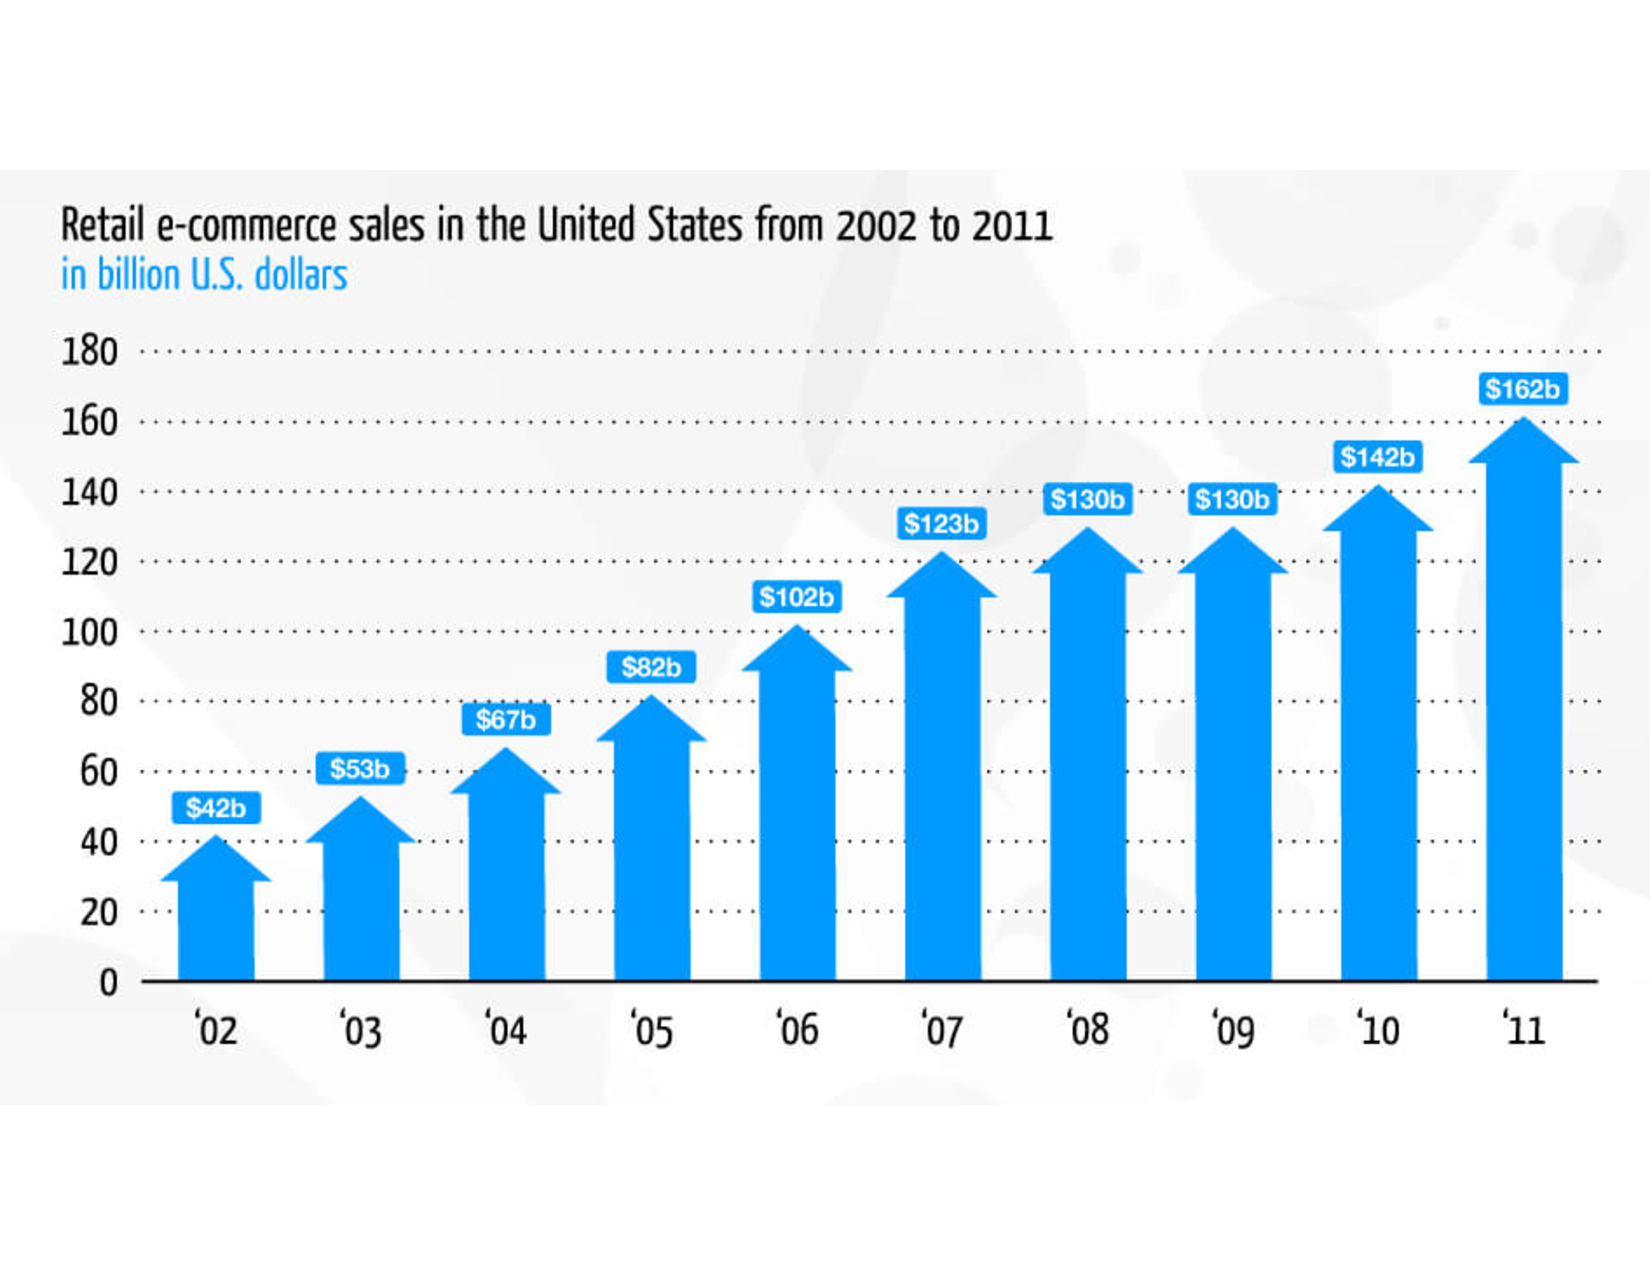
\includegraphics[width=\columnwidth]{eCommerce_chart}}
			\caption{Retail sales in the USA between 2002 and 2011.}
			\label{sales}
		\end{center}
	\vskip -0.2in
\end{figure} 

\begin{figure}[ht]
	\vskip 0.2in
		\begin{center}
			\centerline{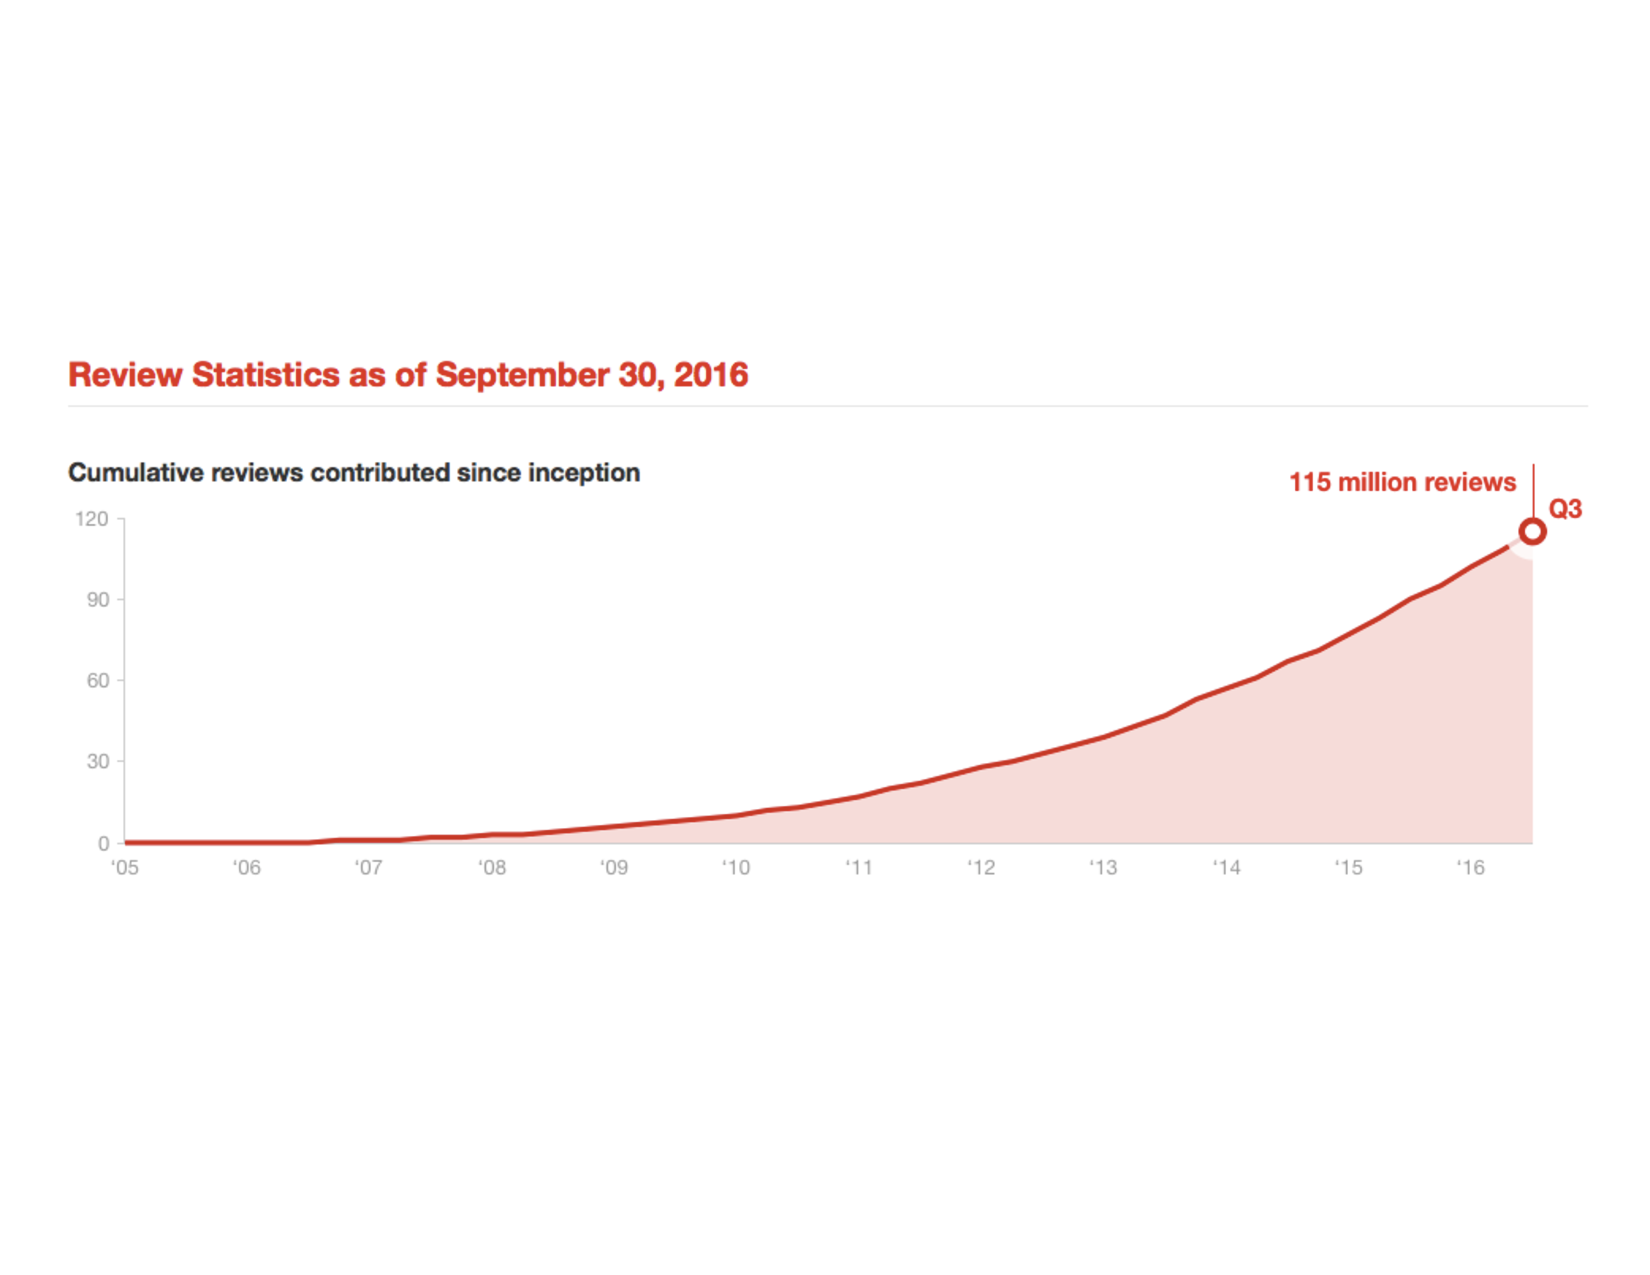
\includegraphics[width=\columnwidth]{yelp_stats}}
			\caption{Yelp Review Statistics}
			\label{yelp}
		\end{center}
	\vskip -0.2in
\end{figure} 


\begin{figure}[ht]
	\centerline{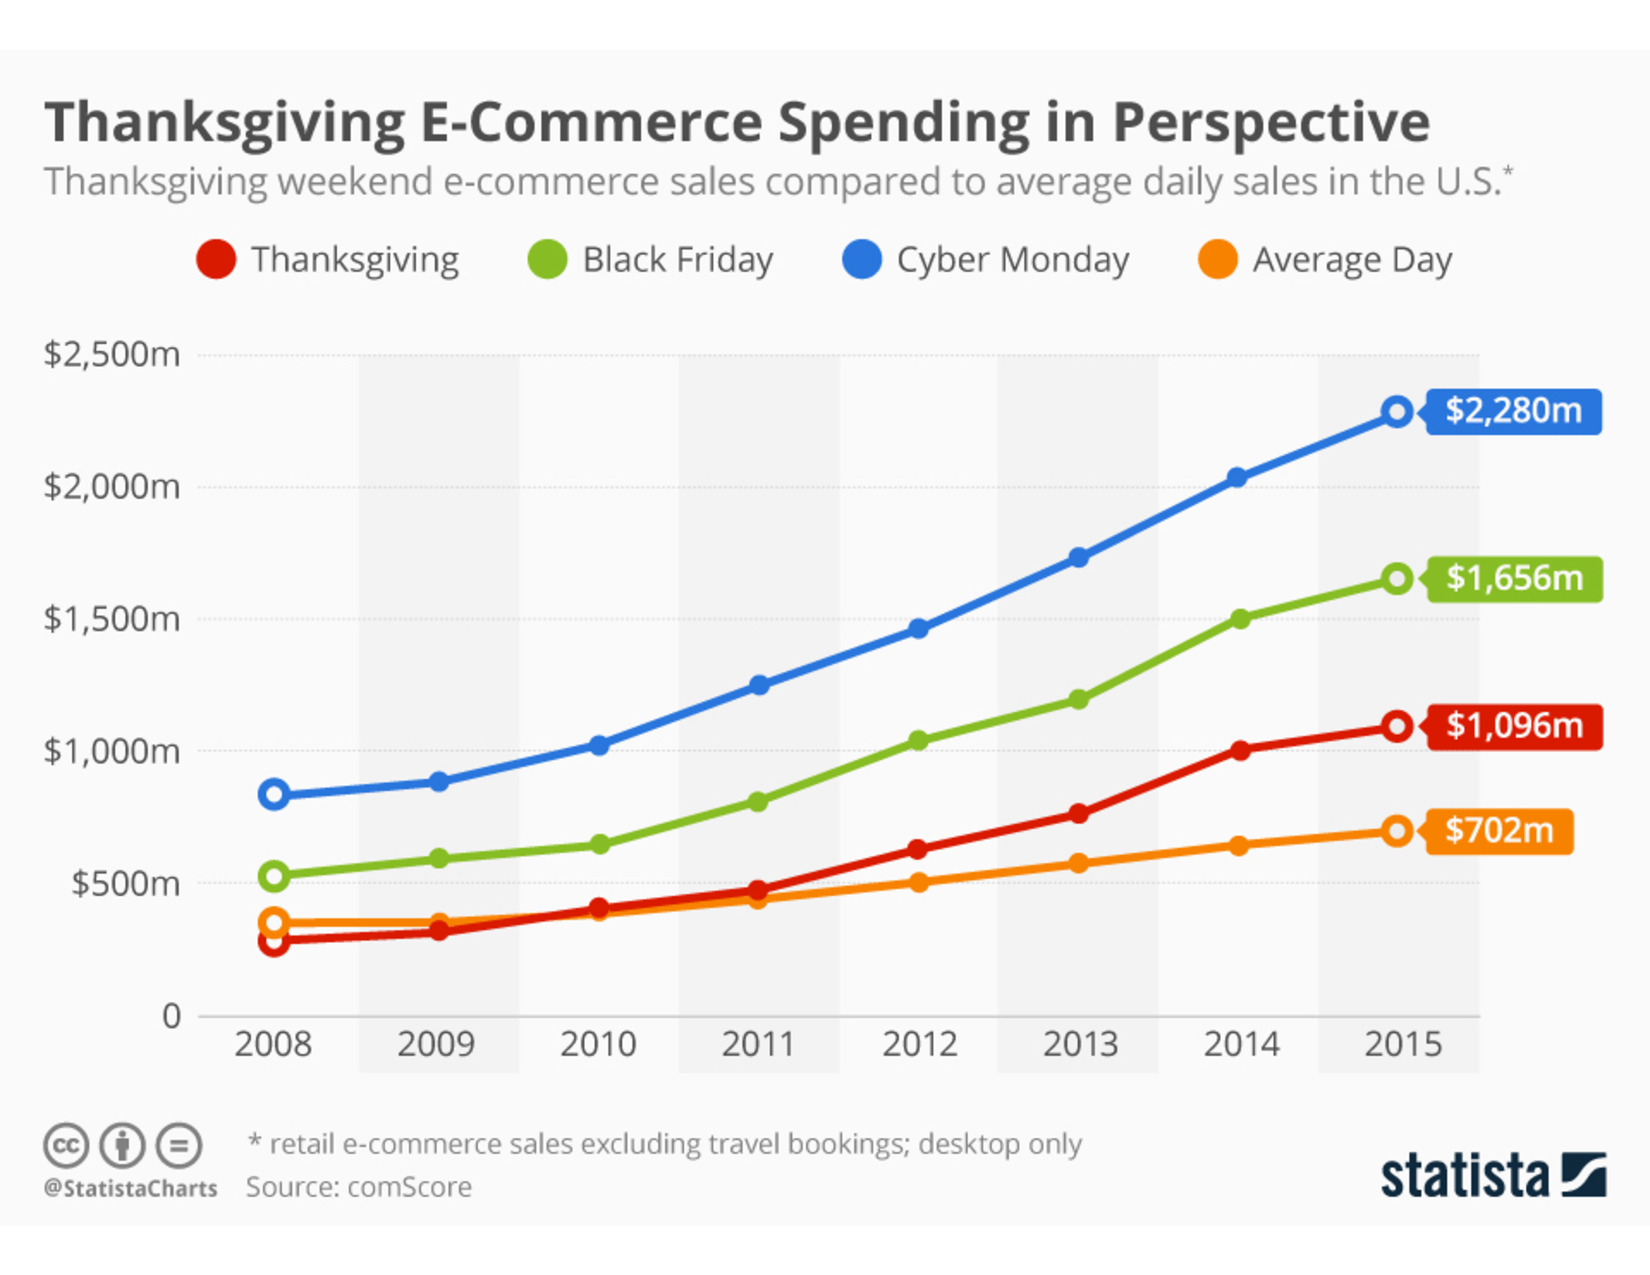
\includegraphics[width=\columnwidth]{Thanksgiving_sales}}
	\caption{eCommerce sales during the Thanksgiving week.}
	\label{thanksgiving}
	\vskip 0.15in
\end{figure} 


\section{Algorithm Formulation} 
	\label{algorithm} 

	In order to perform all the operations we first started off by extracting the required text from the review data file. After this 		the extracted review text were processed into a format which can then be use within the code and identification numbers 		were assigned to every unique words. This list of unique words had to exclude words such as "a", "the" and so on. This 		was done to avoid wrong analyses of the extracted review text. 
	
	For our algorithm we decided to specify the number of topics that we would be using to group the set of documents into 		upfront ( denoted by K ). For our cases we defined 2 as the number of topics.

	For the first part of algorithm we randomly assigned words to one the 2 topics that we have initialized. Along with			generating this topic assignment list, we created two matrices which are :
	\begin{itemize}
	 	\item \textbf{Word-topic matrix :} in other words we created a count of the words being assigned to each of the 2 				topics. 
		\item \textbf{Document-topic matrix :} This is the matrix with the distribution of the topic assignment list.
	\end{itemize}
	
	In every document \textit{d}, we observe every word \textit{w}.  We then chose a topic \textit{t} with the \textit{p(w | t)} $		\times$ \textit{p(t | d)}, denoted by the following mathematical notations:
	
\twocolumn[
\vskip 0.3 in

$$ p( z_i = j \text{ }| \text{ } z_{-i}, w_i, d_i ) = \frac{ C^{WT}{w_ij} + \eta }{ \sum^W{ w = 1 }C^{WT}{wj} + W\eta }\times 			\frac{ C^{DT}{d_ij} + \alpha }{ \sum^T_{ t = 1 }C^{DT}_{d_it} + T\alpha } $$


\vskip 0.3 in

]
where, 

$p(z_i = j)$ : Probability that word i is assigned to topic j.

$z_{-i}$ : Represents topic assignments of every other word.

$w_i$ : Word ID of the $i_{th}$ word.

$d_i$ : Document containing the $i_{th}$ word.

$C^{WT}$ : Word-topic matrix.

$\sum^W_{ w = 1 }C^{WT}_{wj}$ : Total number of words in each topic.

$C^{DT}$ : Document-topic matrix.

$\sum^T_{ t = 1 }C^{DT}_{d_it}$ : Total number of words in document i.

$\eta$ : Parameter to set the topic distribution for the words.

$\alpha$ : Parameter to set the topic distribution for the documents.

$W$ : Total number of words in the set of documents.

$T$ : Number of topics.


After drawing the new topic we update the topic assignment list with newly sampled topic for the word \textit{w}

After that increment the word-topic and document-topic count matrices with the new sampled topic for word \textit{w}.

After we complete learning the topics for \textit{r} iterations iterations, we use the count matrices to obtain the word-topic distribution and document-topic distribution.

LDA assumes that each document is a mixture of all topics, thus after computing the probability that each document belongs to each topic we use this information to see which topic each of the documents belong to and possible words that are associated with each topic.

After understanding the computations we attempted to tune the parameters.

Since the starting point sampling point of dataset is chosen randomly, thus it makes sense to discard the first few iterations. Due to the fact that they most likely do not reflect the properties of distribution accurately. And another parameter is  the number of iterations omitted during the training. This prevents the correlation between samples while iterating.


\section{Feature Engineering} 
	\label{engineer} 

	In order to perform the function of topic modeling we needed a dataset for which we used the review's dataset which was provided in the Yelp dataset. The dataset was found to be large in order to process and obtain results quickly. Due to time constraints it had to be sub-sampled to about 500 reviews. This gave the satisfaction that our results was obtained efficiently on a large enough dataset required to generalize our algorithm.
	
	The primary feature that was required to perform the desired task was review text. Not much else was needed apart from this. Using. the review text we created other parameters which we then used to create a topic model. Some of these were 
	
	\begin{itemize}
		\item{Word-topic matrix}
		\item{Document-topic matrix}
		\item{The various probabilities of occurrences}
	\end{itemize} 

	However we could not use the review text as obtained in the dataset. We had to process the extracted data so that the necessary functions could be applied to it in order to obtain the results. 
	
	In order to obtain and process the data we first had to convert the JSON file into a useable CSV file. Once this was done we sub-sampled the dataset into something that was smaller and would give us a flavor of what we could expect from a larger dataset. 
	
	Once the sub-sampling was complete we created a list of all the words within each review and then removed stop words i.e. words such as "a", "the" and so on... This helped us in forming a list with all the relevant and necessary words which could then be applied in our topic modeling algorithm. 
	
	After removing the stop words we went ahead and labelled the sentences i.e. we implemented topic modeling using the 	LDA algorithm and then classified each subtopic into groups such as Price, Time of the day, Service, etc...
	  
	 We created specific methods within our code to implement the tasks. 
	
\section{Evaluation} 
	\label{eval} 

	Enter the evaluation and parameters used for the evaluation...

\section{Results} 
	\label{result} 

\begin{figure}[ht]
	\centerline{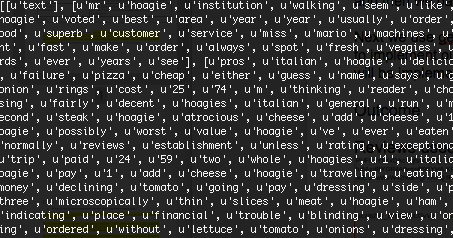
\includegraphics[width=\columnwidth]{preproctext}}
	\caption{Pre-Processed text that will be used for the implementation}
	\label{preproctext}
	\vskip 0.15in
\end{figure} 

\begin{figure}[ht]
	\centerline{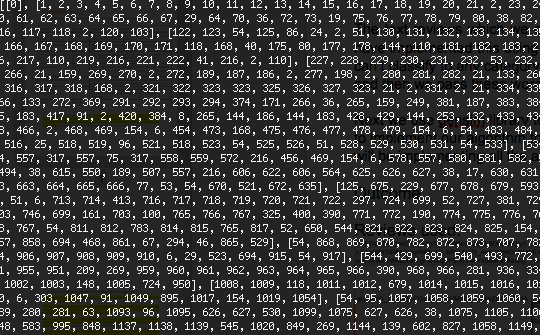
\includegraphics[width=\columnwidth]{tokenized}}
	\caption{Tokenized text}
	\label{tokenized}
	\vskip 0.15in
\end{figure} 

\begin{figure}[ht]
	\centerline{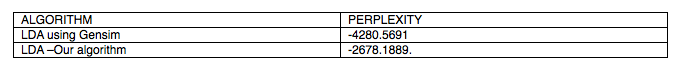
\includegraphics[width=\columnwidth]{lda}}
	\caption{LDA Evaluation result}
	\label{lda}
	\vskip 0.15in
\end{figure} 
 

\section{Challenges}
	\label{challenges}
	
	During the course of the project we encountered a few significant challenges which we eventually were able to over come. Some of the challenges that we encountered were. 
	
	\begin{itemize}
		\item{Understanding the LDA algorithm along with the parameters and the equations necessary for processing of the data}
		\item{Once we got a hold on the topic we had to arrive at a sub-sampled dataset which was large enough to get a good result}
	\end{itemize}
\section{Learning objectives achieved}
	\label{learning}
	Over the course of the project over the last few weeks we achieved a good proficiency in many areas. The highlights of our learning include :
	
	\begin{itemize}
		\item{We gained a good understanding of the Latent Dirichlet Allocation algorithm. Along with the algorithm itself we 				were able to understand it's functioning and the pro's and cons associated with it. 
		
			We were also able to get a good grip on it's implementation.}
		
		\item{It helped us discover and understand new packages available in python. Packages such as gensim and 					pyLDAvis.}
	\end{itemize}
	
	
\section{Deliverables}
	\label{time}
	
	We believe that 8 weeks was a short period for us to work on the project and that more could be done provided we had more time available. A few of the ideas that we had are :
	
	\begin{itemize}
		\item{ To create an API which could then be used to generate ratings based on the review text.}
		\item{ To use the code against a larger dataset with more review texts.}
		\item{ To use the code against different datasets. By this we mean that we intend to use the code against dataset 				obtained from other sites such as Amazon and eBay. This would help verify cross-platform functionality.}
	\end{itemize}

\begin{thebibliography}{9}

 
\bibitem{griffith} 
	T. L. Griffith, M. Steyvers. 
	\textit{Finding Scientific Topics} 	
	PNAS, vol. 10, 6 April - 2004.
 
\bibitem{zhai} 
	Ke Zhai, Jordan Boyd-Graber. 
	\textit{Online Latent Dirichlet Allocation with Infinite Vocabulary} 
	In proceedings, \textit{0th International Conference on Machine Learning}, Atlanta,GA, 2013
	JMLR : W&CP volume 28. Copyright 2013 by the author

\bibitem{lda} 
	D .M. Blei, A. Y. Ng, M. I. Jordan. 
	\textit{Latent Dirichlet Allocation} 
	Journal of Machine Learning Research. 
	January, 2003

\bibitem{crest} 
	Blei, D. M., Griffiths, T. L., Jordan, M. I., & Tenenbaum, J. B. 
	\textit{Hierarchical topic models and the nested Chinese restaurant process} 
	In Advances in Neural Information Processing Systems 16. Cambridge, MA, USA: MIT Press.
	2004

\bibitem{cmu} 
	Erosheva, E. A. 
	\textit{Grade of membership and latent structure models with applications to disability survey data. } 
	Unpublished doctoral dissertation, Department of Statistics, Carnegie Mellon University.

\bibitem{hoffman} 
	Hofmann, T. 
	\textit{Probabilistic Latent Semantic Analysis.} 
	In Proceedings of the Fifteenth Conference on
	Uncertainty in Artificial Intelligence.

\bibitem{zhuang} 
	Zhuang.L, Jing.F, Zhu.X. 
	\textit{Movie Review Mining and Summarization.} 
	CIKM?06, Arlington, VA, USA, 2006.

\bibitem{hum} 
	Hu.M, Liu.B
	\textit{Mining and Summarizing Customer Reviews.} 
	KDD '04, Seattle, WA, USA. 2004

\bibitem{mcauley} 
	McAuley.J, Leskovec.J
	\textit{Hidden Factors and Hidden Topics: Understanding Rating Dimensions with Review Text} 
	In Proceedings of the 7th ACM conference on Recommender systems, Hong Kong, China. 2013

\end{document} 